%%%%%%%%%%%%%%%%%%%%%%%%%%%%%%%%%%%%%%%%%%%%%%%%%%%%%%%%%%%%%%%
% Arithmetic of the clock
% Author: Juan Luis Varona
% http://www.unirioja.es/cu/jvarona/
%%%<
%%%>
% :Title: Arithmetic of the clock
% :Author: Juan Luis Varona
% 
% This example shows the products i times j for
% i and j from 0 to 11 by using arithmetic modulo 12,
% i.e., the so called arithmetic of the clock.
% 
% The results of the products are represented both by
% the color of the clock and by the hand.
% Colors:
\definecolor{clock0}{cmyk}{1,0,0,0} % cyan
\definecolor{clock1}{cmyk}{0.75,0.25,0,0}
\definecolor{clock2}{cmyk}{0.5,0.5,0,0}
\definecolor{clock3}{cmyk}{0.25,0.75,0,0}
\definecolor{clock4}{cmyk}{0,1,0,0} % magenta
\definecolor{clock5}{cmyk}{0,0.75,0.25,0}
\definecolor{clock6}{cmyk}{0,0,5,0.5,0}
\definecolor{clock7}{cmyk}{0,0.25,0.75,0}
\definecolor{clock8}{cmyk}{0,0,1,0} % yellow
\definecolor{clock9}{cmyk}{0.25,0,0.75,0}
\definecolor{clock10}{cmyk}{0.5,0,0.5,0}
\definecolor{clock11}{cmyk}{0.75,0,0.25,0}
% x pos, y pos, color, hand position
\newcommand{\clock}[4]{%
  \begin{scope}[xshift=2.25*#1cm,yshift=2.25*#2cm]
  % \filldraw [fill=#3, line width=1.6pt] (0,0) circle (1cm); % simple fill (unused)
  % \draw[fill] (0,0) circle (1mm); % border (unused)
  \shadedraw [inner color=#3!30!white, outer color=#3!90!black, 
    line width=1.6pt] (0,0) circle (1cm); % disk with shadow and border
  \foreach \angle in {0, 30, ..., 330} 
    \draw[line width=1pt] (\angle:0.82cm) -- (\angle:1cm);
  \foreach \angle in {0,90,180,270}
    \draw[line width=1.3pt] (\angle:0.75cm) -- (\angle:1cm);
  \draw[line width=1.6pt] (0,0) -- (90-30*#4:0.6cm); % the hand 
  \end{scope}
}


\begin{minipage}{3.0in}
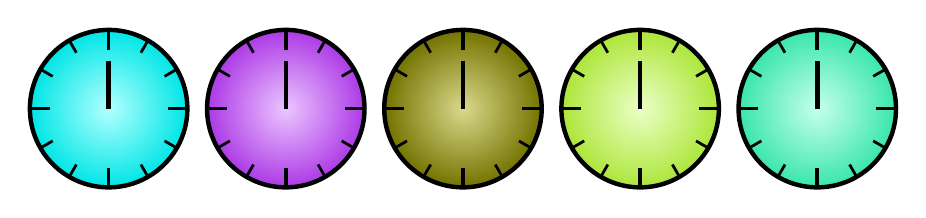
\begin{tikzpicture}[scale=1]

    \clock{0}{0}{clock0}{1*0}; 
    \clock{1}{0}{clock3}{1*0};
    \clock{2}{0}{clock6}{1*0}; 
    \clock{3}{0}{clock9}{1*0};  
    \clock{4}{0}{clock11}{1*0}; 

\end{tikzpicture}%
\end{minipage}

\begin{minipage}{2.0in}
\begin{figure}
\begin{tikzpicture}
    \path[->]<2-> node[special,]
(Requirements) at (0,-4)
{More effective criterions require addtional runtime};
\end{tikzpicture}
\end{figure}
\end{minipage}
